\documentclass[11pt,a4paper]{article}

\usepackage{amsmath}
\usepackage{amssymb}
\usepackage{amsthm}
\usepackage{graphicx}
\usepackage{geometry}
\geometry{margin=2.5cm}
\usepackage{hyperref}
\usepackage{xcolor}
\usepackage{enumitem}

% Custom commands (aligned with long note)
\newcommand{\oper}[1]{\mathcal{#1}}
\newcommand{\vecnorm}[1]{\left\lVert #1 \right\rVert}
\newcommand{\abs}[1]{\left| #1 \right|}
\newcommand{\myfrac}[2]{\frac{#1}{#2}}
\newcommand{\mytilde}[1]{\widetilde{#1}}
\newcommand{\myhat}[1]{\widehat{#1}}
\newcommand{\bm}[1]{\mathbf{#1}}
\newcommand{\cov}{\mathrm{Cov}}
\newcommand{\corr}{\mathrm{Corr}}
\newcommand{\E}{\mathbb{E}}
\newcommand{\Real}{\mathbb{R}}
\newcommand{\erfc}{\mathrm{erfc}}
\newcommand{\Var}{\mathrm{Var}}

% Title and author
\title{\textbf{Short Presentation Note:\\Markov Locality, Diffusion Fill-In, and the First Non-Gaussian Route}}
\author{}
\date{March 2026}

\begin{document}

\maketitle

\begin{abstract}
\noindent
The Gaussian AR(1) benchmark is solved. What remains: how local Markov structure appears in the score, how diffusion reshapes it, how noise erases it. This note presents the strongest benchmark facts, a deterministic control experiment that separates propagation-induced couplings from destroyed Markov locality, and the first non-Gaussian extension (Laplace) with exact Fourier representation and position-dependent score Hessian. Figures are primary; derivations are in the full manuscript.
\end{abstract}

\section{Benchmark and Open Problem}

Consider the AR(1) model:
\[
a_{k+1} = \alpha a_k + \eta_k, \quad \eta_k \sim \mathcal{N}(0, \sigma_\eta^2), \quad |\alpha| < 1,
\]
with prior $a_0 \sim \mathcal{N}(\mu_0, \Sigma_0)$. Under Ornstein--Uhlenbeck noising, the diffused state at time $t$ is:
\[
x_k = e^{-t} a_k + \sqrt{\Delta_t} \, z_k, \quad \Delta_t = 1 - e^{-2t},
\]
with marginal covariance:
\[
\Sigma_t = e^{-2t} \Sigma_0 + \Delta_t \bm{I}.
\]

For Gaussian $p_t(x)$, the score is affine:
\[
S(x,t) = \nabla \log p_t(x) = -Q_t(x - \mu_t),
\]
where $Q_t = \Sigma_t^{-1}$ is the \textit{precision matrix} and $\gamma_t = e^{-2t}/\Delta_t$.

\vspace{0.3cm}
\noindent
\textbf{Two organizing ingredients:}
\begin{enumerate}[label=(\roman*)]
  \item \textbf{Gaussianity:} Affine score, spectral decoupling in eigenbasis.
  \item \textbf{Markovianity:} AR(1) structure makes $Q_0$ \textit{tridiagonal}, encoding only nearest-neighbor interactions.
\end{enumerate}

\vspace{0.3cm}
\noindent
\textbf{Central question:} How does this local Markov structure survive, deform, and disappear in the score under diffusion?

\section{Gaussian Benchmark: The Precision Lifecycle}

\subsection*{Structure and Spectral Dynamics}

The initial precision is tridiagonal:
\[
Q_0 = \begin{pmatrix}
q_0 & -q_1 & 0 & \cdots \\
-q_1 & q_0 & -q_1 & \cdots \\
0 & -q_1 & q_0 & \cdots \\
\vdots & \vdots & \vdots & \ddots
\end{pmatrix}
\]
with all structure concentrated in the first three diagonals. Covariance contracts uniformly:
\[
(\Sigma_t)_{jk} = e^{-2t} (\Sigma_0)_{jk} \quad \text{for } j \neq k.
\]

The precision restructures via spectral decomposition:
\[
Q_t = U \, \mathrm{diag}\left( \frac{1}{e^{-2t}\lambda_i + \Delta_t} \right) U^\top = \frac{1}{\Delta_t} (I + \gamma_t \Sigma_0)^{-1}.
\]

\vspace{0.2cm}
\noindent
\textbf{Coupling distance scales at small times:} Distance-$d$ couplings appear at order $t^{d-1}$,
\[
Q_t = e^{2t} \sum_{m \geq 0} (-c_t)^m Q_0^{m+1}, \quad c_t = e^{2t} - 1.
\]
This geometric series encodes band-by-band fill-in: first neighbors at $O(1)$, second at $O(t)$, third at $O(t^2)$, etc.

\vspace{0.2cm}
\noindent
\textbf{Large-time asymptotics:}
\[
Q_t \approx I - e^{-2t}(\Sigma_0 - I).
\]
The precision becomes nearly identity as diffusion dominates.

\vspace{0.4cm}
\begin{figure}[h!]
\centering

\includegraphics[width=0.45\textwidth]{figures/fig01_sigma0_vs_precision0.pdf}
\hspace{0.05\textwidth}

\includegraphics[width=0.45\textwidth]{figures/fig02_sigma_t_panel.pdf}
\caption{\textbf{Left:} Initial covariance $\Sigma_0$ (dense, rank-full) vs. initial precision $Q_0$ (tridiagonal, Markov). \textbf{Right:} Precision lifecycle: band-by-band fill-in and diffusion-driven relaxation toward identity.}
\label{fig:lifecycle}
\end{figure}

\section{Locality Diagnostics}

To quantify how Markov structure persists or dissolves, we define four observables:

\begin{enumerate}
  \item \textbf{Tridiagonal mass:} $T_1(t) = \sum_{i,j: |i-j| \leq 1} Q_t[i,j]^2 / \|Q_t\|_F^2$.
  \item \textbf{Effective bandwidth:} $b_{0.95}(t) = \min \{d : \sum_{|i-j| \leq d} Q_t[i,j]^2 \geq 0.95 \|Q_t\|_F^2\}$.
  \item \textbf{Interaction range:} $\bar{\xi}(t) = \sum_{d \geq 1} d \cdot P(|i-j| = d)$ where $P$ is the band-mass distribution.
  \item \textbf{Neighbor score correlation:} $\rho_1(t) = \corr(S_k, S_{k+1})$, read directly from $Q_t$.
\end{enumerate}

Since $\cov(S_t) = Q_t$ (the precision itself), these observables fully characterize locality in the score. The posterior mean is:
\[
\E[a \mid X_t = x] = \mu_0 + G_t(x - \mu_t), \quad G_t = e^{-t} \Sigma_0 Q_t.
\]

\begin{figure}[h!]
\centering

\includegraphics[width=0.95\textwidth]{figures/fig10_locality_observables.pdf}
\caption{\textbf{Four-panel locality diagnostics:} Tridiagonal mass fraction $T_1(t)$ decays; bandwidth $b_{0.95}(t)$ grows; interaction range $\bar{\xi}(t)$ increases; neighbor correlation $\rho_1(t)$ vanishes. Diffusion simultaneously fills the precision and decorrelates it.}
\label{fig:locality}
\end{figure}

\section{Deterministic Control Experiment}

To isolate how Markov structure is destroyed by diffusion, we study a deterministic analogue with no stochastic innovation noise:
\[
a_k = \alpha^k A_0, \quad \Sigma_0^{\mathrm{det}} = \sigma_0^2 \bm{v} \bm{v}^\top, \quad \bm{v} = (1, \alpha, \ldots, \alpha^K)^\top.
\]

By Sherman--Morrison, after noising:
\[
Q_t^{\mathrm{det}} = \frac{1}{\Delta_t} I - C(t) \bm{v} \bm{v}^\top.
\]

\textbf{Key observation:} The precision becomes \textit{globally dense immediately}, even for arbitrarily small $t > 0$. The rank-one structure of $\Sigma_0^{\mathrm{det}}$ induces global couplings purely through \textit{propagation}, independent of diffusion destroying Markov locality.

\vspace{0.3cm}
\noindent
\textbf{Noncommuting limits:}
\begin{itemize}
  \item $(t \to 0, \sigma_\eta^2 > 0)$: Tridiagonal $Q_0$.
  \item $(\sigma_\eta^2 = 0, t > 0)$: Rank-one-modified identity, globally dense.
\end{itemize}

This experiment cleanly separates \textit{diffusion-destroyed Markov locality} from \textit{propagation-induced global coupling}.

\begin{figure}[h!]
\centering

\includegraphics[width=0.95\textwidth]{figures/fig09_deterministic_vs_stochastic_precision.pdf}
\caption{\textbf{Stochastic (left) vs. deterministic (right) precision matrices:} Stochastic AR(1) shows band-by-band fill-in and eventual diffusion-driven relaxation. Deterministic model produces global coupling from propagation alone, illustrating that the source of global structure can be separated from diffusion destruction of local Markov form.}
\label{fig:det_control}
\end{figure}

\section{First Non-Gaussian Extension: Laplace}

The Gaussian benchmark is solved. We now take the first step beyond Gaussianity.

\subsection*{Model and Fourier Representation}

Let $a_{k+1} = \alpha a_k + \varepsilon_k$ with $\varepsilon_k \sim \mathrm{Laplace}(0, b)$. The characteristic function is $\myhat{f}(q) = \frac{1}{1 + b^2 q^2}$, making $\mathrm{Laplace}(0,b)$ the low-frequency tangent to $\mathcal{N}(0, 2b^2)$.

Under diffusion, the exact Fourier representation is:
\[
\Phi_t(\xi) = \exp\left( -\frac{\Delta_t \|\xi\|^2}{2} \right) \cdot \Phi_0(e^{-t} \xi).
\]

For $K=1$ (scalar $a_0$), the posterior density after noising is computed via Laplace--Gaussian convolution:
\[
h(y; \tilde{b}, \sigma^2) = \frac{1}{4\tilde{b}} \exp\left( \frac{\sigma^2}{2\tilde{b}^2} \right) \left[ \exp(y/\tilde{b}) \, \erfc(\cdots) + \exp(-y/\tilde{b}) \, \erfc(\cdots) \right],
\]
followed by 1D Gaussian integration over $a_0$. The exact formula is closed-form, validated against Monte Carlo.

\subsection*{Score and Position-Dependent Hessian}

The score $S(x, t) = \nabla \log p_t(x)$ is now \textbf{nonlinear}. Critically, the score Hessian:
\[
H_t(x) = -\nabla^2 \log p_t(x)
\]
\textbf{depends on $x$}. In the Gaussian case, $H_t \equiv Q_t$ is constant. Here, the "effective precision" varies with location in data space.

For $K=2$, the Markov chain structure is preserved: the density factors as a chain of 1D integrals, each solvable by the same closed-form Laplace--Gaussian recipe.

\vspace{0.3cm}
\noindent
\textbf{Monte Carlo validation:} Numerical integration confirms the exact computation to machine precision.

\begin{figure}[h!]
\centering
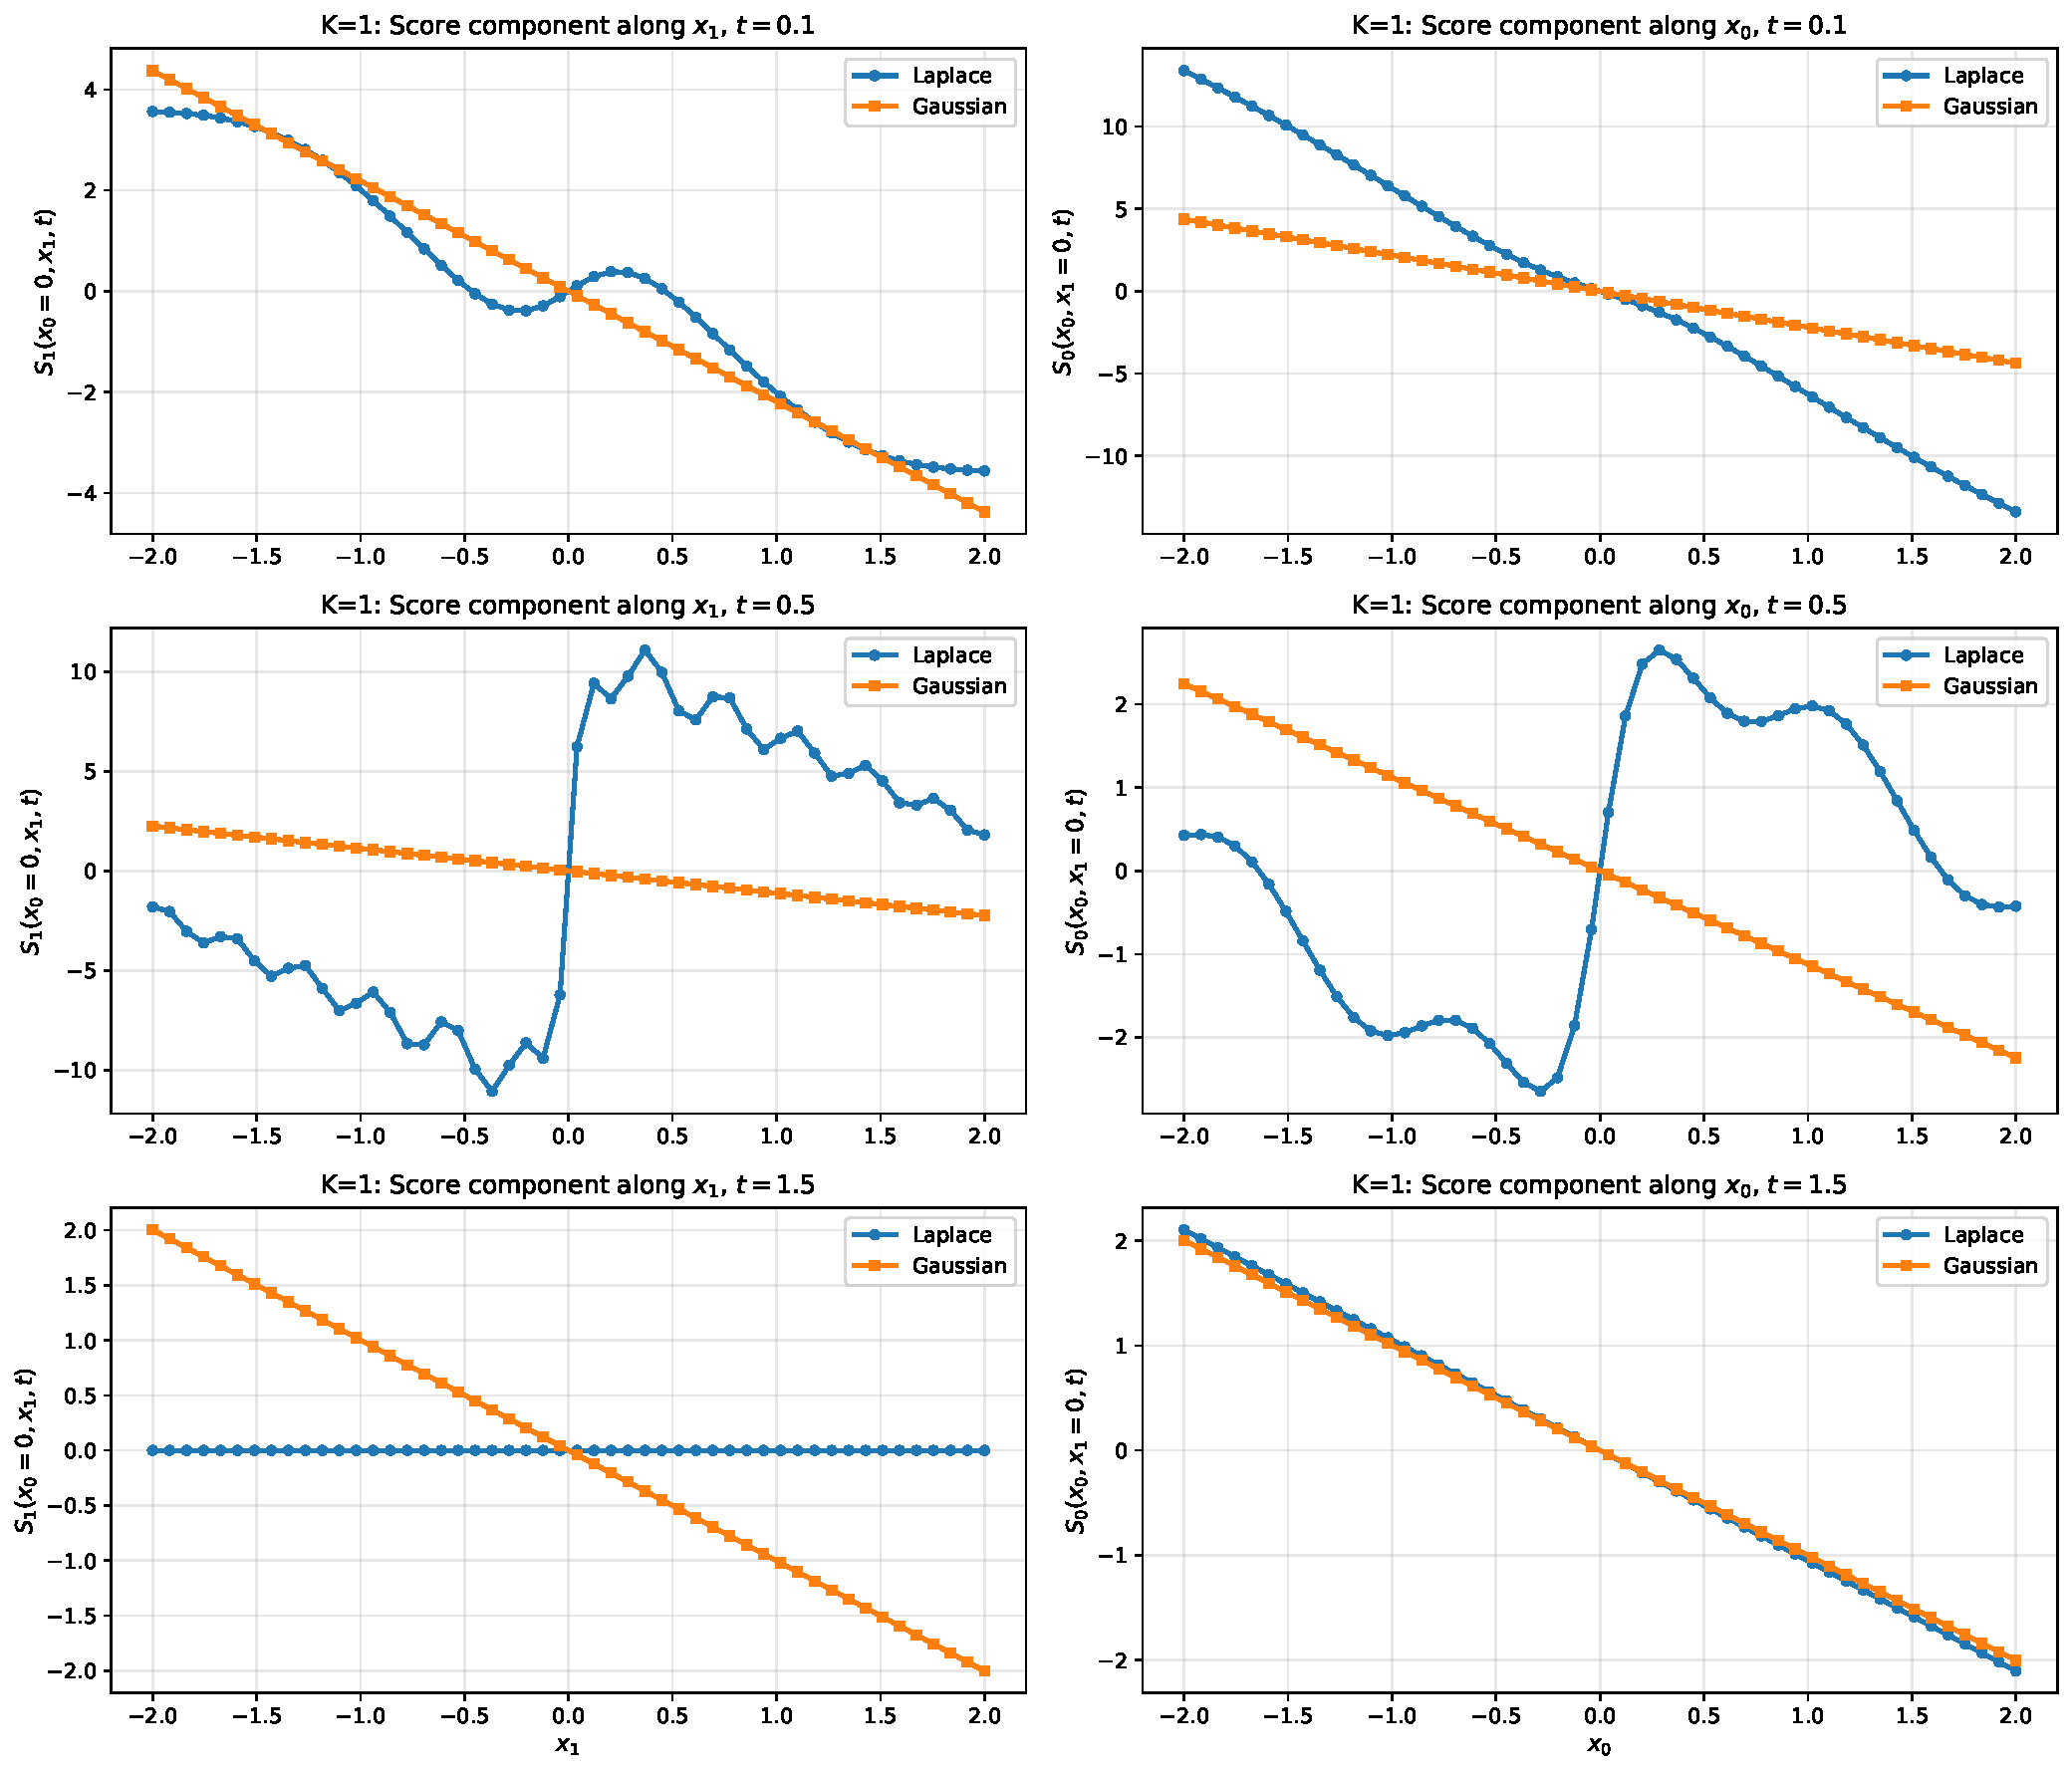
\includegraphics[width=0.45\textwidth]{figures/fig13_k1_score_laplace_vs_gaussian.pdf}
\hspace{0.05\textwidth}
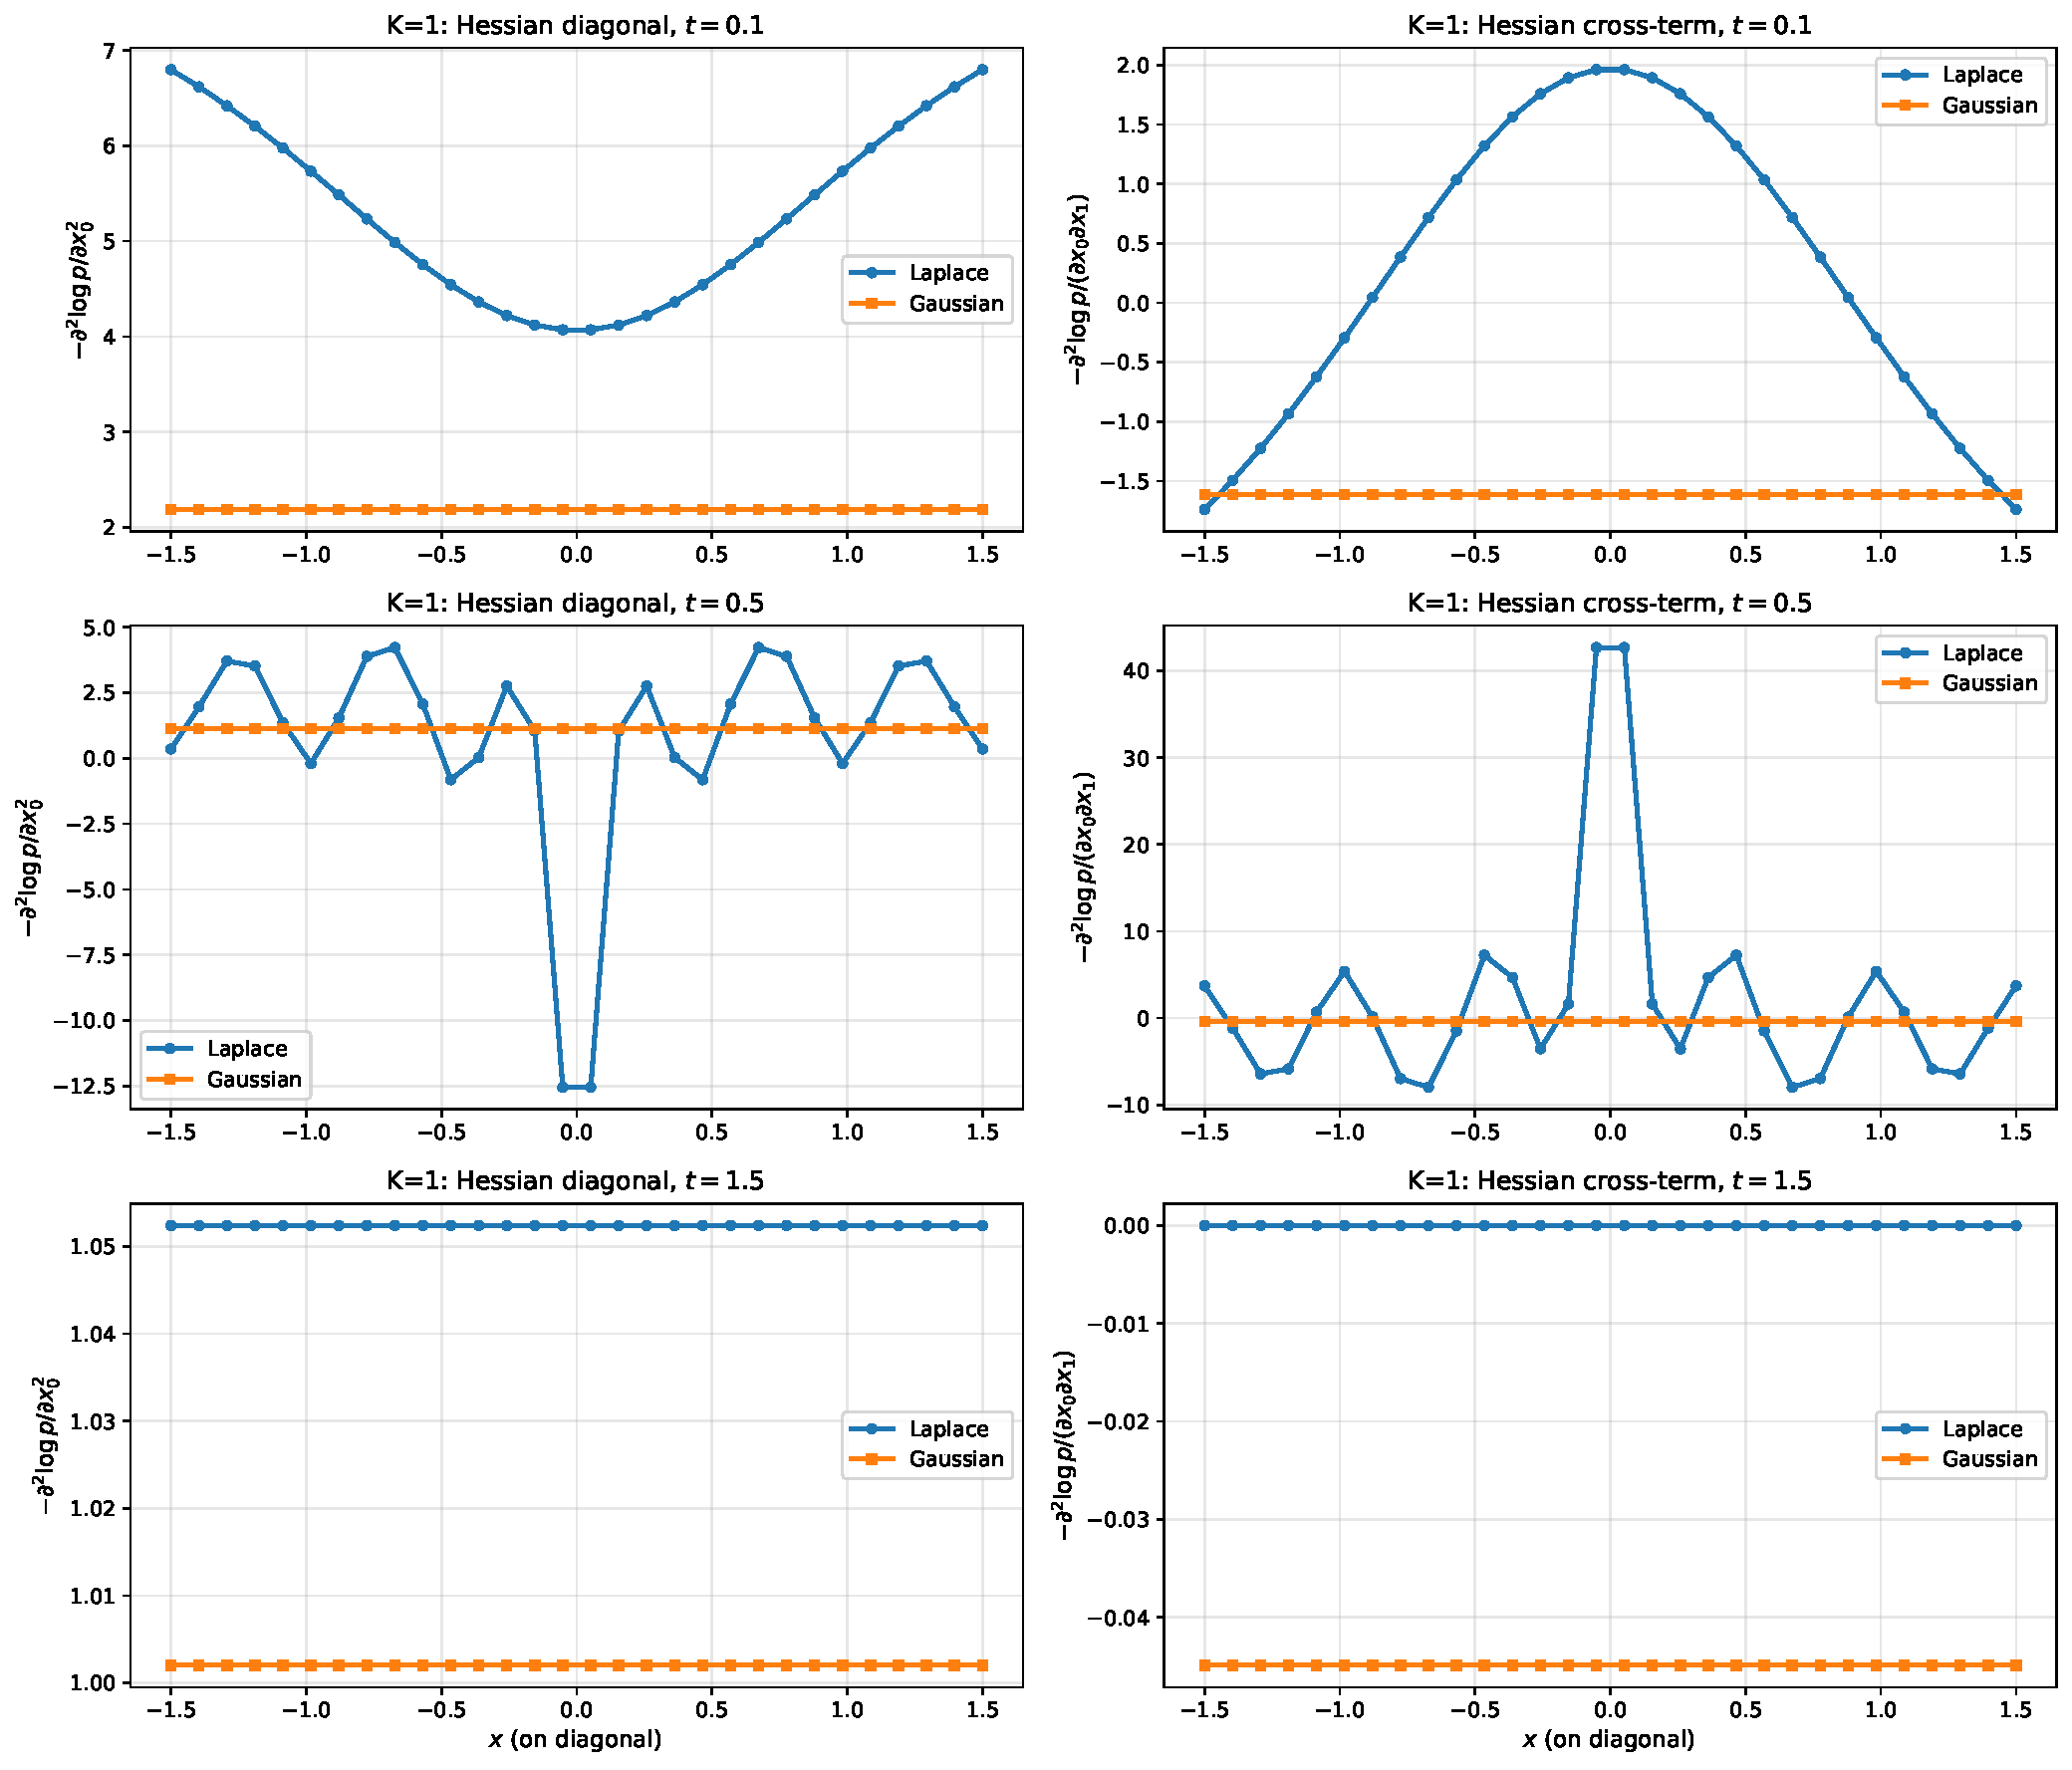
\includegraphics[width=0.45\textwidth]{figures/fig14_k1_score_hessian.pdf}
\caption{\textbf{Left:} Score in Laplace model (blue, nonlinear) vs. Gaussian (orange, affine) for $K=1$. \textbf{Right:} Score Hessian $H_t(x)$ (effective precision) is position-dependent in Laplace; constant identity-like in Gaussian (dashed). This $x$-dependence is the hallmark of non-Gaussian score structure.}
\label{fig:laplace}
\end{figure}

\section{Takeaways and Next Steps}

\begin{enumerate}
  \item \textbf{Markov structure lives in precision, not covariance:} $Q_0$ is tridiagonal while $\Sigma_0$ is dense.

  \item \textbf{Band-by-band fill-in:} Distance-$d$ couplings enter at order $t^{d-1}$. Small-time expansion encodes the geometric series $Q_t = e^{2t} \sum_{m \geq 0} (-c_t)^m Q_0^{m+1}$.

  \item \textbf{Intermediate regime captured by locality observables:} Tridiagonal mass, bandwidth, interaction range, and neighbor correlation quantify the transition from local to global structure.

  \item \textbf{Deterministic benchmark separates mechanisms:} Global couplings can arise from propagation alone; diffusion's destruction of Markov locality is a distinct effect.

  \item \textbf{Laplace model: first exact non-Gaussian extension:} Fourier representation, closed-form 1D integrals, and validated numerics enable systematic non-Gaussian analysis.

  \item \textbf{Score Hessian becomes position-dependent:} In Laplace, $H_t(x) \neq \text{const}$, replacing the global effective precision of the Gaussian case with a local, data-dependent curvature.

  \item \textbf{Next direction:} Systematically study band mass of $H_t(x)$ as a function of $(x, t)$ and extend to higher-order non-Gaussian models (e.g., Student-$t$, mixture innovations).
\end{enumerate}

\vspace{0.5cm}
\noindent
\textbf{Key insight:} The Gaussian AR(1) diffusion score is solved. The first non-Gaussian extension shows that locality becomes both space-dependent and model-dependent. This opens the door to understanding how diffusion reshapes and erases Markov structure in realistic, non-Gaussian settings.

\section*{References}

\begin{enumerate}
  \item Ornstein, L. S., \& Uhlenbeck, G. E. (1930). On the theory of the Brownian motion. \textit{Phys. Rev.}
  \item Song, Y., Sohl-Dickstein, J., Kingma, D. P., Kumar, A., Ermon, S., \& Poole, B. (2020). Score-based generative modeling through stochastic differential equations. \textit{ICLR}.
  \item Ho, J., Jain, A., \& Abbeel, P. (2020). Denoising diffusion probabilistic models. \textit{NeurIPS}.
  \item Anderson, B. D. O. (1982). Reverse-time diffusion equation models. \textit{Stoch. Process. Appl.}
  \item Koehler, P., \& Gribonval, R. (2021). Learning to denoise. \textit{SIAM Rev.}
  \item Huang, S. -W., et al. (2024). Diffusion-based generative models with learnable rank-adaptive noise injection.
  \item Long, Z., Lu, Y., Dong, B., \& others (2024). On the implicit bias of score matching in denoising.
\end{enumerate}

\end{document}
